\documentclass[MTech]{iitmdiss}

\usepackage{times}
\usepackage{setspace}
\usepackage{amsmath,amsthm,amssymb,amsfonts}
\usepackage{verbatim}
\usepackage{floatrow}
\usepackage{fullpage}
\usepackage{listings}
%\usepackage{txfonts,pxfonts,amsfonts}
\usepackage[usenames,dvipsnames]{xcolor}


\usepackage{xcolor}
\usepackage{caption}
\usepackage{subfig}
\usepackage{graphicx}

\usepackage[square]{natbib}
\usepackage[colorlinks=true,linkcolor=black]{hyperref}
%\usepackage{hyperref} % hyperlinks for references.
\usepackage[all]{hypcap}
\usepackage{complexity}
\usepackage[named]{algo}
%\usepackage{algpseudocode}

\newtheorem{thm}{Theorem}
\newtheorem{problem}{Problem}
\newtheorem{corr}{Corollary}
\newtheorem{lma}{Lemma}
\newtheorem{case}{Case}
\newtheorem{rmrk}{Remark}
\newtheorem{prp}{Proposition}
\newtheorem{dfn}{Definition}
\newtheorem{qn}{Question}
\newtheorem{att}{Attempt}
\newtheorem{ex}{Example}
\newtheorem{flaw}{Flaw in Attempt}
\usepackage{bm}
\usepackage{xcolor}
\usepackage{float}
\xdefinecolor{gray}{rgb}{0.4,0.4,0.4}
\xdefinecolor{blue}{RGB}{58,95,205}% R's royalblue3; #3A5FCD

% Strut macros for skipping spaces above and below text in tables. 
\def\abovestrut#1{\rule[0in]{0in}{#1}\ignorespaces}
\def\belowstrut#1{\rule[-#1]{0in}{#1}\ignorespaces}

\def\abovespace{\abovestrut{0.20in }}
\def\aroundspace{\abovestrut{0.20in}\belowstrut{0.10in}}
\def\belowspace{\belowstrut{0.10in}}
%%%%%%%%%%%%%%%%%%%%%%%%%

\lstset
{
	numbers=left,
    breaklines=true,
    postbreak=\raisebox{0ex}[0ex][0ex]{\ensuremath{\color{red}\hookrightarrow\space}}
}

\def\thesistitle{}
\def\thesisauthor{D Akshay Rangasai}


\begin{document}
\bibliographystyle{iitm}
%%%%%%%%%%%%%%%%%%%%%%%%%%%%%%%%%%%%%%%%%%%%%%%%%%%%%%%%%%%%%%%%%%%%%% 
% Title page

\title{\thesistitle}

\author{\thesisauthor}

\date{May 2015}
\department{Mechanical Engineering}

%\nocite{*}
\begin{singlespace}
\maketitle 
\end{singlespace} 

%%%%%%%%%%%%%%%%%%%%%%%%%%%%%%%%%%%%%%%%%%%%%%%%%%%%%%%%%%%%%%%%%%%%%%
% Certificate
\certificate

\vspace*{0.5in}

\noindent This is to certify that the thesis entitled {\bf {\thesistitle}}, 
submitted by {\bf {\thesisauthor}}, to the Indian Institute of Technology, 
Madras, for the award of the degree of {\bf Master of Technology}, 
is a bona fide record of the research work carried out by him under my
supervision. The contents of this thesis, in full or in parts, have not been
submitted to any other Institute or University for the award of any degree or
diploma.

\vspace*{1.4in}
\hspace*{-0.25in}
\begin{minipage}{0.5\textwidth}
\begin{singlespace}
\noindent {\bf Krishnan Balasubramanian} \\
\noindent Research Guide \\ 
\noindent Professor \\
\noindent Dept. of Mechanical Engineering\\
\noindent IIT-Madras, 600 036 \\
\end{singlespace}
\end{minipage}
\begin{minipage}{0.5\textwidth}
\begin{singlespace}
\noindent {\bf L Vijayaraghavan} \\
\noindent Research Co-Guide \\ 
\noindent Professor \\
\noindent Dept. of Mechanical Engineering\\
\noindent IIT-Madras, 600 036 \\
\end{singlespace}
\end{minipage}
\vspace*{0.20in}
\noindent Place: Chennai\\ 
Date:

%%%%%%%%%%%%%%%%%%%%%%%%%%%%%%%%%%%%%%%%%%%%%%%%%%%%%%%%%%%%%%%%%%%%%%
\acknowledgements
I want to thank myself for this completely pointless endeavour and my parents for paining me constantly about this. This is in the end, quite depressing.
%%%%%%%%%%%%%%%%%%%%%%%%%%%%%%%%%%%%%%%%%%%%%%%%%%%%%%%%%%%%%%%%%%%%%%
% Abstract

\abstract
Most materials have two regimes of operation when it comes to the relationship between stress and strain of the material, namely linear and non-linear. while phenomenon and material characterization in the linear regime of operation is pretty well understood, the non-linear regime is not as well understood. This is an intriguing part of the problem as materials that undergo plastic deformation and fatigue loading operate under this non-linear regime, and characterization of these properties help in various manufacturing processes.

This study aims to statistically model and extract relevant parameters to measure non-linearity and its effects on a material by the use of ultrasonic waves, which provide a high strain rate, but very low strain, which is ideal to test the material without changing any of its properties at the current state. We first characterize parameters through harmonics generation and then proceed to non-linear wave mixing, a technique which gives us spatial specificity in our measurements. 

The forward model was first built by creating a Finite Difference Time Domain (FDTD) solution to a set of differential equations that represent two dimensional non-linear wave propagation in an isotropic solid medium in a euclidean coordinate system. Wave mixing was simulated using a transverse and a longitudinal wave mixing in collinear path, with a phased array simulated as the transducer. Sensitivity analysis was performed for this solution and this formed the basis of our inverse model that helped predict material parameters.

The inverse model for the forward model was first built using linear regression and the results were compared with a statistical learning technique. We used Gaussian Process modelling to model the predictive model, which we further used to build the inverse model. To evaluate the model, noise was added to the measurements at various Signal to Noise Ratio (SNR) and the error percentage was measured. This model proved to be sufficient for the inverse model. From this, we could effectively estimate model parameters from wave mixing measurements.

The thesis further explores the directions this work could take along with the applications of the said techniques. By expanding on the dimensionality and complexity of the problem, we can effectively use this technique to monitor as well as improve manufacturing processes. 
\pagebreak

%%%%%%%%%%%%%%%%%%%%%%%%%%%%%%%%%%%%%%%%%%%%%%%%%%%%%%%%%%%%%%%%%
% Table of contents etc.

\begin{singlespace}
\tableofcontents
\thispagestyle{empty}

\listoftables
\addcontentsline{toc}{chapter}{LIST OF TABLES}
\listoffigures
\addcontentsline{toc}{chapter}{LIST OF FIGURES}
\end{singlespace}

\pagebreak


%The main text will follow from this point so set the page numbering
%to arabic from here on.
\pagenumbering{arabic}
%%%%%%%%%%%%%%%%%%%%%%%%%%%%%%%%%%%%%%%%%%%%%%%%%%
% Introduction.
%\input{misc.tex}
%\input{questions.tex}
\chapter{Introduction}

The subject of the present work deals with the propagation, non-linear mixing effects of high-frequency shear and longitudinal waves which help us characterize material properties. This section is a brief introduction containing the background, outline and applications of the presented work.

\section{Background}
The stress-strain curve for most ductile materials starts in a linear relationship and moves into a non-linear relationship with a few invariants that define the said relationship. Determining these constants is of great use to characterize the material and predict its behaviour under various conditions and also optimize processes with respect to these constants. While the physical relationship between the linear constants and their estimation has been studied to a great extent, the non-linear constants are more difficult to estimate. Our work aims to estimate these non-linear constants through statistical estimation techniques.

\subsection{The stress-strain curve}
\begin{center}
\begin{figure}[ht]
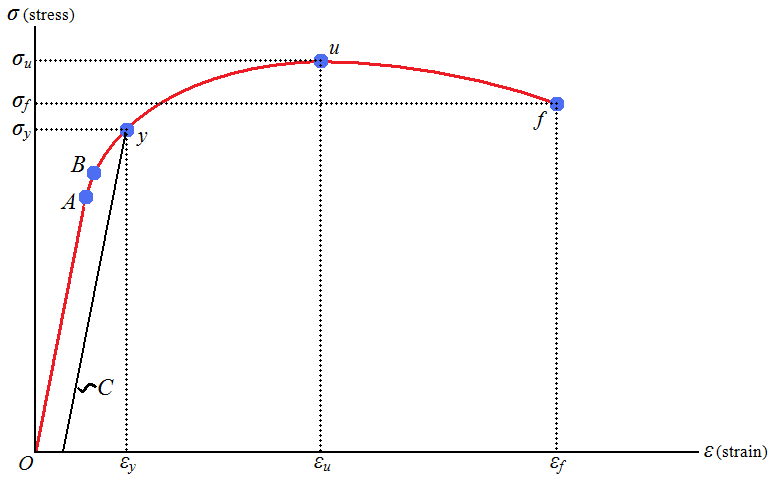
\includegraphics[scale=0.45]{images/chapter_1/stressstrain.png}
\caption{The Stress Strain Curve for a Typical Material}
\end{figure}
\end{center}
The significant points from fig 1.1.1 are as follows:
\begin{enumerate}
\item A - Proportional Limit
\item B - Elastic Limit
\item y - Yield Point
\item u - Ultimate Tensile Strength
\item f - Fracture point
\end{enumerate}
\subsection{Non-Destructive Testing}
There are multiple methods of figuring out the elastic constants of a material, most significant of them being destructive methods, where the material is stressed to its Ultimate Tensile Strength and then, a curve is fit to get the second order constants of the material. This results in the material specimen being destroyed and deemed useless. This method is good for laboratory conditions, but not in a real-world scenario.

To account for this, we employ a method of Non-Destructive testing using ultrasonics. Ultrasonic waves have the characteristic of extremely high strain rates, but the magnitude of strain itself is minimal, and the changes to material properties are thus negligible. These high strain rates result in interesting phenomenon occurring, which in turn helps us estimate parameters of the material, without any physical damage to the specimen.

\subsection{Wave Propagation and Mixing}
One of the main concepts that are used in this study are that of wave propagation in solid media and mixing of waves in linear and non-linear zones. To solve the differential equations involved, we use FDTD simulations. We employed multiple solvers to evaluate the equations and multiple approaches to solve the problem. This will be discussed in detail in upcoming chapters.

\subsection{Statistical Inversion and Learning}
The forward model is inverted by using purely statistical techniques. We employ various techniques from Support Vector Machines (SVM), Gaussian Mixture Models (GMMs), and Gaussian Processes. The mathematics and results will be discussed in detail in the coming chapters.
\section{Outline of the Report}
This report is organized into 6 chapters.
\begin{enumerate}

\item The current chapter gives a basic introduction to the project and explains very briefly what we hope to achieve and techniques we've employed with a little bit of background information.

\item Chapter 2 deals with Literature Review and what we worked on and the subsequent results of the same with reasons as to what method we finally adopted and why with a discussion about the same.

\item Chapter 3 describes the construction of the FDTD model for the forward problem and the collinear wave mixing approach that is taken by us and describes the problem and solution in detail.

\item Chapter 4 explores the sensitivity analysis of our constructed forward model with respect to various parameters of interest and and exploratory analysis of the inverse model.

\item Chapter 5 validates the inverse model and also describes the pitfalls of the model. We make the model more real world friendly and check its performance.

\item Chapter 6 summarizes our work and has a section on how this project can be pursued along with suggestions for experimental validation.
\end{enumerate}
\section{Applications of present work}
The present work has wide range of uses from aircraft industry to the shipping industry. A manufacturing specific application of this current technique will be in the estimation of material parameters in forming process and cold working processes where materials undergo plastic deformation. 

This technique will help us understand material deformation better and give us a physical insight into what the constants mean and at the same time help improve existing processes and diagnose issues in current processes.  

\chapter{Literature Review}
\section{Introduction}
to first understand the problem at hand and look at how to proceed, a literature survey was undertaken by us. We scoured through multiple scientific journals and used them as markers for our work. Due to the relative similarity of this problem to that faced in photonics/optics, many papers from an Electrical/Quantum Mechanical background were found. A few papers that developed theory rigorously were also looked at. Below, we shall list out the most important papers in our survey and also explain what each paper contributed to this project. Post that, we describe the approach we plan to take to tackle the problem at hand.


\section{Paper Review}

The first paper is from 1971, from an old soviet journal \cite{zarem} This paper develops the theory from first principles and attempts to solve it using relatively older numerical techniques. This paper clearly explains non-linear phenomena in solid. This paper formed the base of our future work, and our first simulation solver was based on the ideas given in this paper. The paper, besides the rigorous mathematical treatment of the subject at hand, also delves into phonon interaction in materials in brief.

With this background, we derive that there are only a few modes of mixing that is accepted in a material, and these criteria converge whichever approach you take to treat the subject. With a basic phonon treatment of the subject matter, the nuances of wave mixing are also discussed. This is very important and acts as the base on which the rest of the project is built.

This paper was implemented initially, and the results were quite accurate, but this didn't quite serve the purpose of what we set out to do and thus we switched our starting point.

%Put table of Wave Mixing and possible modes and shit. Diagrams also

\begin{figure}
\begin{center}
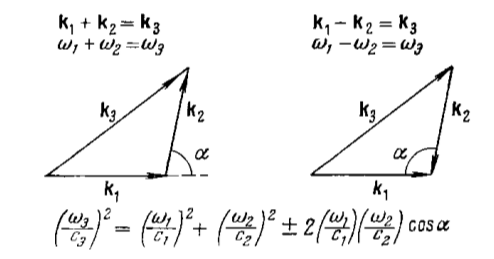
\includegraphics[scale=0.5]
{images/chapter_2/directions_noncollinear.png}
\caption{Direction of resultant wave\cite{zarem}}
\end{center}
\end{figure}

\begin{figure}
\begin{center}
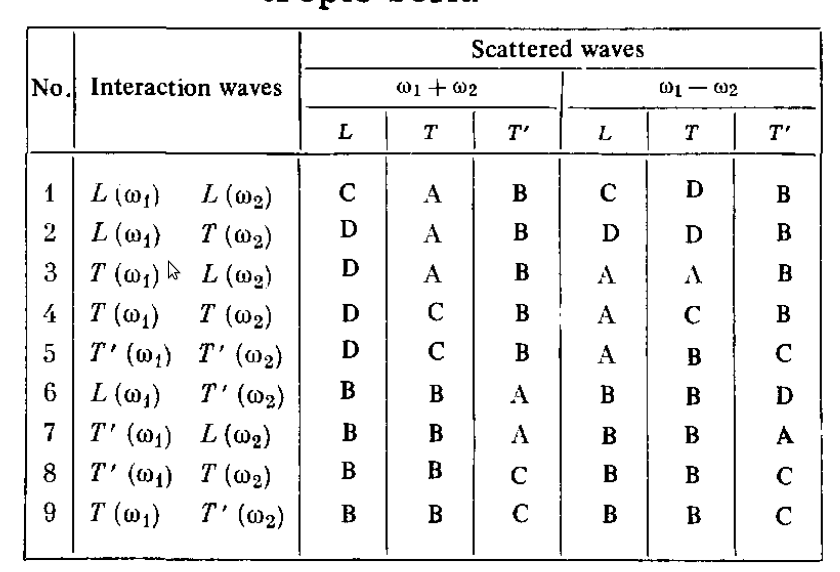
\includegraphics[scale=0.5]
{images/chapter_2/interaction.png}
\caption{Forbidden Modes of Wave Mixing \cite{zarem}}
\end{center}
\end{figure}

The second paper that was pursued post this was a paper on three phonon interaction and a quantum(light) analogue applied to solid material. This paper further expounded on acceptable modes of mixing and also the direction and wave-characteristics of the resulting wave. However, the approach taken by the authors in the paper seemed far too advanced for our purposes and thus this paper was used for experimental setup than the starting point for our work.


The third paper of great significance was that by Liu \cite{Liu}. This paper had a very classical treatment of the governing equation and its solution in a 2 Dimensional collinear environment. The paper was not too advanced and proved useful as our starting point in the simulations. 

The differential equations derived are in two dimensions and could be solved easily. an FDTD method approach was taken over any other approach due to the flexibility of FDTD methods. This paper formed the basis of the forward model and sensitivity analysis. Based on this and a few other readings, we decided to take this approach to tackle the problem.

\begin{figure}
\begin{center}
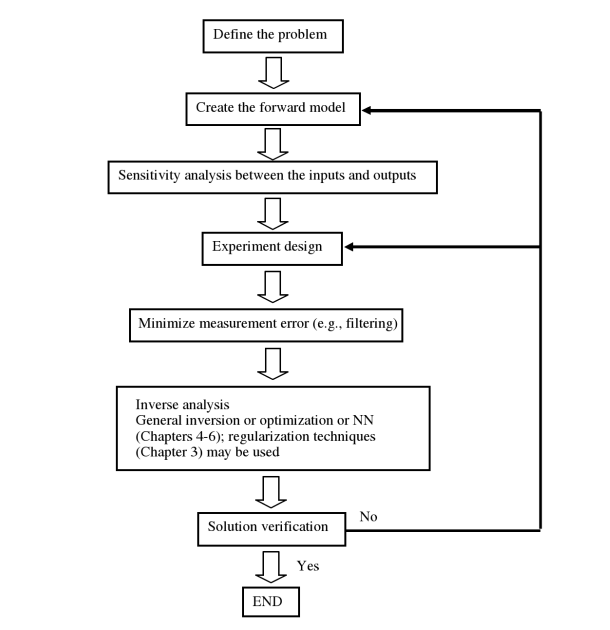
\includegraphics[scale=1]
{images/chapter_2/mthodology_generic.png}
\caption{Generic Methodology of this Project}
\end{center}
\end{figure}

For the inverse model, most of the literature was read from Bishop \cite{bishop} and a few other PhD thesis. This marks the end of literature survey and implementation details of the project
\chapter{Future Work}

%%%%%%%%%%%%%%%%%%%%%%%%%%%%%%%%%%%%%%%%%%%%%%%%%%%%%%%%%%%%
% Appendices.
%\appendix
\chapter{Appendix}
\input{appendix.tex}
\section{Solver Code}
\lstinputlisting[language=Python]{../solver.py}
\pagebreak
\section{Problem Formulation code Code}
\lstinputlisting[language=Python]{../formulation.py}
\pagebreak
\lstinputlisting[language=Python]{../data.py}
\pagebreak
\lstinputlisting[language=Python]{../constants.py}
\pagebreak
\lstinputlisting[language=Python]{../framework.py}
\pagebreak
\lstinputlisting[language=Python]{../sensitivity_analysis.py}
\pagebreak
\lstinputlisting[language=Python]{../GMM_regression.py}
\pagebreak
\lstinputlisting[language=Python]{../defaults.py}
% Bibliography.
\pagebreak
\begin{singlespace}
  \begin{small}
	\bibliography{bibliography}
  \end{small}
\end{singlespace}

%%%%%%%%%%%%%%%%%%%%%%%%%%%%%%%%%%%%%%%%%%%%%%%%%%%%%%%%%%%%

\end{document}
